\documentclass[11pt]{article}
\usepackage[a4paper,margin=16mm]{geometry}
\usepackage{amsmath,amssymb}
\usepackage{tikz}
\usetikzlibrary{arrows.meta,positioning,fit,backgrounds,calc}
\usepackage[hidelinks]{hyperref}

% ---- node styles -------------------------------------------------------
\tikzset{
  lem/.style   ={draw,rounded corners,align=center,font=\small,
                 inner sep=3pt,fill=blue!6},
  def/.style   ={draw,rounded corners,align=center,font=\small,
                 inner sep=3pt,fill=gray!8},
  head/.style  ={draw,rounded corners,align=center,font=\small\bfseries,
                 inner sep=4pt,fill=orange!14},
  mlib/.style  ={draw,dashed,rounded corners,align=center,font=\footnotesize,
                 inner sep=3pt,fill=green!6},
  ar/.style    ={-{Stealth[length=2mm]},shorten >=1pt,shorten <=1pt},
}
\newcommand{\lc}[1]{\texttt{#1}}

\begin{document}
\begin{center}
  {\large\bfseries Dependency DAG of $(1)\Rightarrow(2)$}\\[1mm]
  {\footnotesize headline \lc{eqn2\_of\_eqn1}: for $x\neq0$, equation
  $(1)\Rightarrow \ell_k(c,x)=0$ \; (edge $A\to B$: ``$A$ proved using $B$'')}
\end{center}

% =======================================================================
% The DAG
% =======================================================================
\begin{center}
\resizebox{\textwidth}{!}{%
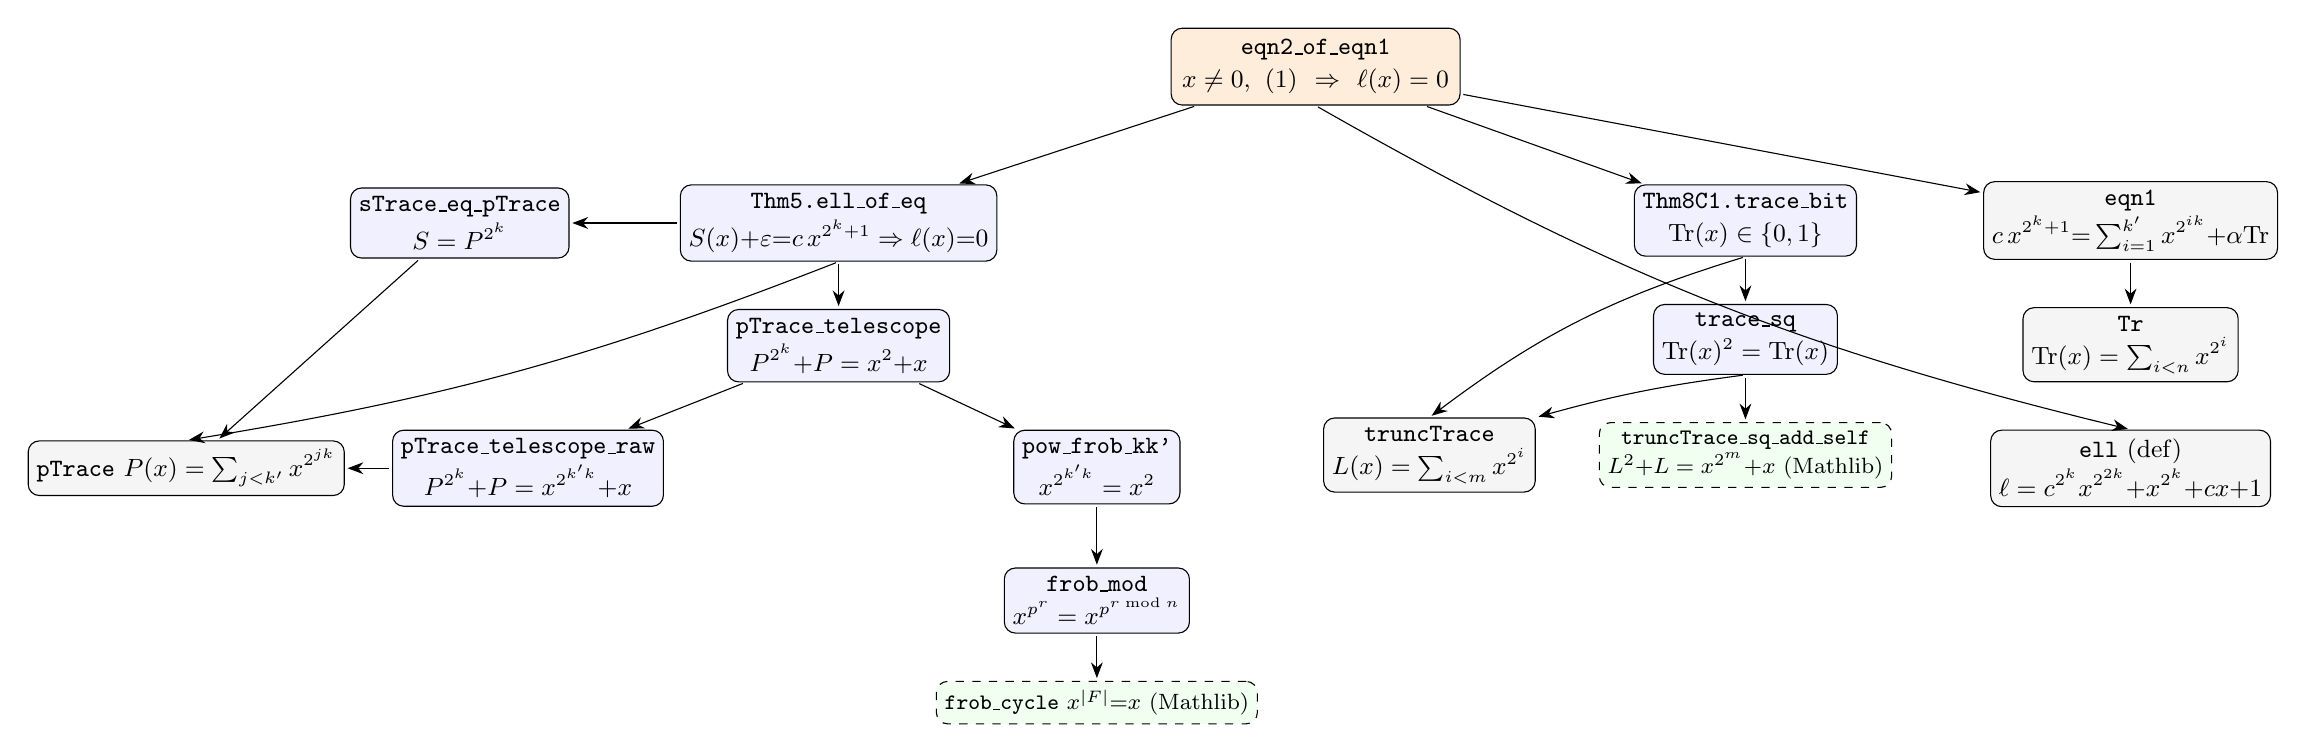
\begin{tikzpicture}[node distance=6mm and 8mm]
% headline
\node[head] (H) {\lc{eqn2\_of\_eqn1}\\[1pt]
  $x\neq0,\ (1)\ \Rightarrow\ \ell(x)=0$};

% ---- branch 1 (left): telescoping / Artin--Schreier -> ell_of_eq ------
\node[lem,below left=10mm and 22mm of H] (ELL) {\lc{Thm5.ell\_of\_eq}\\[1pt]
  $S(x){+}\varepsilon{=}c\,x^{2^k{+}1}\Rightarrow\ell(x){=}0$};
\node[lem,below=of ELL] (TEL) {\lc{pTrace\_telescope}\\[1pt]
  $P^{2^k}{+}P=x^2{+}x$};
\node[lem,below left=of TEL] (RAW) {\lc{pTrace\_telescope\_raw}\\[1pt]
  $P^{2^k}{+}P=x^{2^{k'k}}{+}x$};
\node[lem,below right=of TEL] (FKK) {\lc{pow\_frob\_kk'}\\[1pt]
  $x^{2^{k'k}}=x^2$};
\node[lem,below=8mm of FKK] (FMOD) {\lc{frob\_mod}\\[1pt]$x^{p^r}=x^{p^{r\bmod n}}$};
\node[mlib,below=6mm of FMOD] (FCYC) {\lc{frob\_cycle} $x^{|F|}{=}x$ (Mathlib)};
\node[lem,left=14mm of ELL] (SEQ) {\lc{sTrace\_eq\_pTrace}\\[1pt]$S=P^{2^k}$};
\node[def,left=6mm of RAW] (PT) {\lc{pTrace} $P(x)=\sum_{j<k'}x^{2^{jk}}$};

% ---- branch 2 (right): trace parity -> trace_bit ---------------------
\node[lem,below right=10mm and 22mm of H] (TB) {\lc{Thm8C1.trace\_bit}\\[1pt]
  $\mathrm{Tr}(x)\in\{0,1\}$};
\node[lem,below=of TB] (TSQ) {\lc{trace\_sq}\\[1pt]$\mathrm{Tr}(x)^2=\mathrm{Tr}(x)$};
\node[mlib,below=of TSQ] (TSAS) {\lc{truncTrace\_sq\_add\_self}\\[1pt]
  $L^2{+}L=x^{2^m}{+}x$ (Mathlib)};
\node[def,left=8mm of TSAS] (TT) {\lc{truncTrace}\\[1pt]$L(x)=\sum_{i<m}x^{2^i}$};

% ---- branch 3 (far right): definitions -------------------------------
\node[def,right=16mm of TB] (E1) {\lc{eqn1}\\[1pt]$c\,x^{2^k{+}1}{=}\sum_{i=1}^{k'}x^{2^{ik}}{+}\alpha\mathrm{Tr}$};
\node[def,below=of E1] (TR) {\lc{Tr}\\[1pt]$\mathrm{Tr}(x)=\sum_{i<n}x^{2^i}$};
\node[def,below=of TR] (ELLDEF) {\lc{ell} (def)\\[1pt]$\ell=c^{2^k}x^{2^{2k}}{+}x^{2^k}{+}cx{+}1$};

% ---- edges ------------------------------------------------------------
\draw[ar] (H) -- (ELL);
\draw[ar] (H) -- (TB);
\draw[ar] (H) -- (E1);
\draw[ar] (H.south) to[bend right=8] (ELLDEF.north);

\draw[ar] (ELL) -- (TEL);
\draw[ar] (ELL) -- (SEQ);
\draw[ar] (ELL.south) to[bend left=6] (PT.north);
\draw[ar] (TEL) -- (RAW);
\draw[ar] (TEL) -- (FKK);
\draw[ar] (RAW) -- (PT);
\draw[ar] (SEQ) -- (PT);
\draw[ar] (FKK) -- (FMOD);
\draw[ar] (FMOD) -- (FCYC);

\draw[ar] (TB) -- (TSQ);
\draw[ar] (TB.south) to[bend right=10] (TT.north);
\draw[ar] (TSQ) -- (TSAS);
\draw[ar] (TSQ.south) to[bend right=4] (TT.north east);

\draw[ar] (E1) -- (TR);
\end{tikzpicture}}
\end{center}

\begin{center}\footnotesize
\tikz\node[def,inner sep=2pt]{def};\ definition\quad
\tikz\node[lem,inner sep=2pt]{lemma};\ project lemma\quad
\tikz\node[mlib,inner sep=2pt]{Mathlib};\ rests on Mathlib\quad
\tikz\node[head,inner sep=2pt]{headline};
\end{center}

\bigskip
% =======================================================================
% Step-by-step, with Dobbertin text
% =======================================================================
\noindent\textbf{The three inputs and their Dobbertin source.}
The single step $(1)\Rightarrow(2)$ is the opening of the proof of
Theorem~1 in Dobbertin, \emph{Kasami Power Functions, Permutation
Polynomials and Cyclic Difference Sets}.  Verbatim (equations~(1),~(2)):

\begin{quote}\itshape\small
``\dots we shall show that for each fixed $c\in L$, the equation
\[ c\,x^{2^k+1}=\sum_{i=1}^{k'}x^{2^{ik}}+\alpha\,\mathrm{Tr}(x) \tag{1}\]
has at most one solution in $L$.\ Adding the $2^k$-th power of this
equation to itself we get \dots\ and consequently
\[ \ell(x)=c^{2^k}x^{2^{2k}}+x^{2^k}+cx+1=0. \tag{2}\]
Note that $\ell(x)=0$ if and only if
$c\,x^{2^k+1}+\sum_{i=1}^{k'}x^{2^{ik}}+\alpha\,\mathrm{Tr}(x)=0$ or $1$.''
\end{quote}

\noindent The Lean proof realises ``adding the $2^k$-th power to itself''
by an Artin--Schreier telescoping, and the ``$=0$ or $1$'' by the fact
that $\mathrm{Tr}(x)$ is a bit.

\medskip
\noindent\textbf{(A) Telescoping branch} $\to$ \lc{Thm5.ell\_of\_eq}
(the real content of $(1)\Rightarrow(2)$):
\begin{itemize}\itemsep1pt
\item \lc{sTrace\_eq\_pTrace}: $S(x)=P(x)^{2^k}$, with
      $P(x)=\sum_{j=0}^{k'-1}x^{2^{jk}}$, $S(x)=\sum_{i=1}^{k'}x^{2^{ik}}$.
\item \lc{pTrace\_telescope\_raw}: $P(x)^{2^k}+P(x)=x^{2^{k'k}}+x$ (char $2$, no field needed).
\item \lc{pow\_frob\_kk'}: if $kk'\equiv1\ (\mathrm{mod}\ n)$ then $x^{2^{k'k}}=x^2$
      (uses \lc{frob\_mod}\,$\to$\,\lc{frob\_cycle}, i.e.\ $x^{|F|}=x$).
\item \lc{pTrace\_telescope}: hence $P(x)^{2^k}+P(x)=x^2+x$ (Artin--Schreier form).
\item \lc{bit\_pow}: $\varepsilon\in\{0,1\}\Rightarrow\varepsilon^{2^m}=\varepsilon$.
\item \lc{ell\_of\_eq}: from $S(x)+\varepsilon=c\,x^{2^k+1}$ ($\varepsilon\in\{0,1\}$, $x\neq0$),
      raising $P=(x^2+x)+c\,x^{2^k+1}+\varepsilon$ to the $2^k$ power and dividing by $x^{2^k}$
      gives $\ell(x)=0$.
\end{itemize}

\noindent\textbf{(B) Trace-parity branch} $\to$ \lc{Thm8C1.trace\_bit}
(this is the ``$=0$ or $1$'' above): $\mathrm{Tr}(x)\in\{0,1\}$.
\begin{itemize}\itemsep1pt
\item \lc{truncTrace}: $L(x)=\sum_{i=0}^{m-1}x^{2^i}$ (the trace, def).
\item \lc{truncTrace\_sq\_add\_self}: $L(x)^2+L(x)=x^{2^m}+x$.
\item \lc{trace\_sq}: on $\mathbb F_{2^n}$, $\mathrm{Tr}(x)^2=\mathrm{Tr}(x)$ (uses $x^{|F|}=x$).
\item \lc{trace\_bit}: an idempotent in a field is $0$ or $1$.
\end{itemize}

\noindent\textbf{(C) Definitions branch} (\lc{Defs.lean}):
\lc{eqn1} is equation~(1) cleared of denominators; \lc{ell} is
$\ell(x)$ of~(2); \lc{Tr}$(x)=\sum_{i<n}x^{2^i}$.

\medskip
\noindent\textbf{Module-level DAG.}
\begin{center}
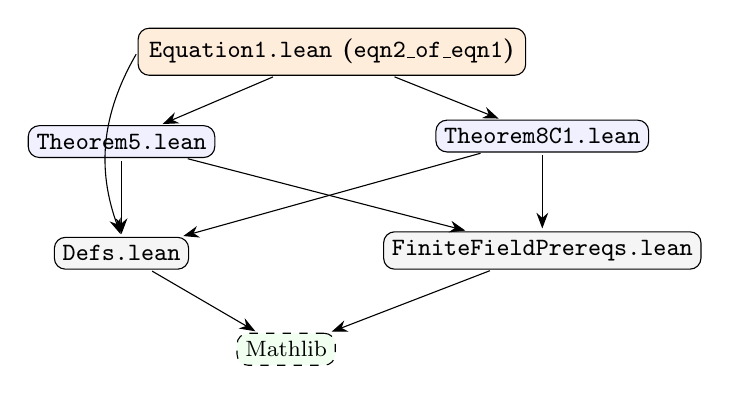
\begin{tikzpicture}[node distance=5mm and 9mm,every node/.style={font=\footnotesize}]
\node[mlib] (M) {Mathlib};
\node[def,above left=8mm and 6mm of M] (D) {\lc{Defs.lean}};
\node[def,above right=8mm and 6mm of M] (F) {\lc{FiniteFieldPrereqs.lean}};
\node[lem,above=10mm of D] (T5) {\lc{Theorem5.lean}};
\node[lem,above=10mm of F] (T8) {\lc{Theorem8C1.lean}};
\node[head,above=8mm of $(T5)!0.5!(T8)$] (EQ) {\lc{Equation1.lean} (\lc{eqn2\_of\_eqn1})};
\draw[ar](D)--(M); \draw[ar](F)--(M);
\draw[ar](T5)--(F); \draw[ar](T8)--(F);
\draw[ar](T5)--(D); \draw[ar](T8)--(D);
\draw[ar](EQ)--(T5); \draw[ar](EQ)--(T8);
\draw[ar](EQ.west) to[bend right=25] (D.north);
\end{tikzpicture}
\end{center}

\noindent\textbf{Not on this path.}
\lc{Theorem8Trace.lean}, \lc{Q1General.lean} and the full
\lc{theorem\_1}, \lc{theorem\_1\_case1}, \lc{theorem\_1\_case2}
bijectivity machinery are \emph{not} used by \lc{eqn2\_of\_eqn1}: the
single step $(1)\Rightarrow(2)$ needs only \lc{Thm5.ell\_of\_eq} and
\lc{Thm8C1.trace\_bit} plus the definitions.

\end{document}
